\documentclass[letter,12pt]{article}
\usepackage[letterpaper,right=1in,left=1in,top=1in,bottom=1in]{geometry}
\usepackage{setspace}

\usepackage[utf8]{inputenc}   % allows input of special characters from keyboard (input encoding)
\usepackage[T1]{fontenc}      % what fonts to use when printing characters       (output encoding)
\usepackage{amsmath}          % facilitates writing math formulas and improves the typographical quality of their output
\usepackage[hyphens]{url}     % adds line breaks to long urls
\usepackage[pdftex]{graphicx} % enhanced support for graphics
\usepackage{tikz}             % Easier syntax to draw pgf files (invokes pgf automatically)
\usetikzlibrary{arrows}

\usepackage{mathptmx}           % set font type to Times
\usepackage[scaled=.90]{helvet} % set font type to Times (Helvetica for some special characters)
\usepackage{courier}            % set font type to Times (Courier for other special characters)

\usepackage[longnamesfirst, sort]{natbib}\bibpunct[]{(}{)}{,}{a}{}{;} % handles biblio and references 

\usepackage{rotating}         % sideway tables and figures that take a full page
\usepackage{caption}          % allows multipage figures and tables with same caption (\ContinuedFloat)

\usepackage{dcolumn}          % needed for apsrtable and stargazer tables from R to compile
\usepackage{arydshln}         % dashed lines in tables (hdashline, cdashline{3-4}, 
                              %see http://tex.stackexchange.com/questions/20140/can-a-table-include-a-horizontal-dashed-line)
                              % must be loaded AFTER dcolumn, 
                              %see http://tex.stackexchange.com/questions/12672/which-tabular-packages-do-which-tasks-and-which-packages-conflict


\newcommand{\mc}{\multicolumn}

%% TO ADD NOTES IN TEXT, PUT % BEFORE THE ONE YOU WANT DISABLED
\usepackage[disable]{todonotes}                            % no show
%\usepackage[colorinlistoftodos, textsize=small]{todonotes} % show notes
\newcommand{\emm}[1]{\todo[color=red!15, inline]{\textbf{Eric:} #1}}
\newcommand{\vp}[1]{\todo[color=green!15, inline]{\textbf{Vale:} #1}}
\newcommand{\ges}[1]{\todo[color=blue!15, inline]{\textbf{Ges:} #1}}

\usepackage{xr} % allows cross-ref to other file
\externaldocument{urge15appendix}

%% %for submission: sends figs, tables, and footnotes to last pages
%% \RequirePackage[nomarkers,nolists]{endfloat}     % sends tables and figures to the end
%% \RequirePackage{endnotes}                        % turns fn into endnotes; place \listofendnotes where you want 
%%                                                  %the endnotes to appear (it must be after the last endnote).
%% \let\footnote=\endnote
%% \newcommand{\listofendnotes}{
%%    \begingroup
%%    \parindent 0pt
%%    \parskip 2ex
%%    \def\enotesize{\normalsize}
%%    \theendnotes
%%    \endgroup
%% }
%% 
%% % for submission: drop page numbers when producing title page
%% \pagenumbering{gobble} % Remove page numbers (and reset to 1)
%% \pagenumbering{arabic}% Arabic page numbers (and reset to 1)


% agradecimientos
%% Vidal Mendoza RA
%% Eugenio Solís RA
%% Sonia Kuri RA
%% Ana Lu RU

\setcitestyle{citesep={;}}

\begin{document}

\title{Speach in Mexico's Cámara de Diputados}
\author{Eric Magar \\ Instituto Tecnológico Autónomo de México}
\date{\today}
\maketitle

\newpage

\begin{abstract}
\noindent Text as data: speaches in lower chamber of Mexico's federal Congress. Analysis covers three pre-midterm election legislative terms since 2006. Argument, findings.\footnote{{Data and supporting materials necessary to reproduce the numerical results in the article are available in the following repository (\url{https://github.com/emagar/legdeb}). Supplementary material for this article is available in the appendix in the online edition.}}
\newline
\newline
\textbf{Keywords}: Speach, Congress, presidentialism, Mexico 
\end{abstract}

\newpage

\doublespacing

\section{Introduction}

\section{Paste in paper}

\subsection{Terminology}

%DONE 3. In terms of window of observation/time period under study: we don’t have a particular guideline for this. Please use the window of observation that you believe is more representative of the politics of legislative debate in your country. Ideally we would like each chapter to include several legislative periods, but we are pragmatic here, considering data availability.

- A *Legislature* is an elected chamber for a legislative term, called a Congress in the U.S. Concurrent with presidential elections the chamber of deputies renovates in whole, and again at the presidential mid-term. Diputados remain three years in office and were single term-limited up to 2021. The 2021 mid-term election will be the first since 1932 to allow incumbents on the ballot, a major change in Mexican legislative politics. Analysis includes the 60th, 62nd, and 64th Legislatures (the Mexican Congress relies on Roman numerals to distinguish Legislatures since the second half of the Nineteenth century).

- Legislative years break into two *ordinary periods*, one covering the months of September through December, inclusive, another February through April, also inclusive. *Extraordinary periods* may be convened during the recess in order to consider a specific bill. Analysis aggregates each member's speeches in the duration of a given period (merging together all extraordinary periods that year, if any). So members in a legislative year like 2012-13 (that had no extraordinary periods) have two word aggregates in the dataset, one for each ordinary period; in a year like 2013-14 (that did), they have three word aggregates in the data. Periods are the units of observation in the analysis. 

- A *plenary session* (or simply a session) is a specific date in the calendar when diputados met. During ordinary periods, sessions are usually held on Tuesdays and Thursdays, and may be scheduled in other weekdays if the Jucopo so decides. Diputados met on forty and thirty-one days in the first and second ordinary periods of 2013-14, respectively, and nine days in extraordinary periods, for a yearly total of eighty session days. (A session in North-American legislative parlance is a Mexican period.)

\subsection{The dependent variables}

Descriptive statistics

\singlespacing
\begin{footnotesize}
\begin{verbatim}
* * Descriptives for diputados vs presiding officers * *
> print(summ)
$mean
   Group.1  dv.nword ev.pot.dys dv.nword.by.dy
1     dips  7539.702   150.8411       48.21666
2 pres.off 65215.062   188.8500      395.45338

$median
   Group.1 dv.nword ev.pot.dys dv.nword.by.dy
1     dips     3677        180       26.37005
2 pres.off    46710        182      258.64011

$sd
   Group.1 dv.nword ev.pot.dys dv.nword.by.dy
1     dips 14811.50   73.40782       79.27871
2 pres.off 63481.32   79.74391      501.86471

$min
   Group.1 dv.nword ev.pot.dys dv.nword.by.dy
1     dips        0          1        0.00000
2 pres.off     3141         32       19.64286

$max
   Group.1 dv.nword ev.pot.dys dv.nword.by.dy
1     dips   242434        522       1212.170
2 pres.off   320155        522       3563.254
\end{verbatim}
\end{footnotesize}
\doublespacing

\subsection{N speakers}

\begin{figure}
  \centering
    \caption{Average marginal effects from model 3. Dots report how the probability of an urgent bill changes in response to a unit change in each independent variable, all else at mean values; bars are 95-percent confidence intervals.}\label{F:avgMg}
    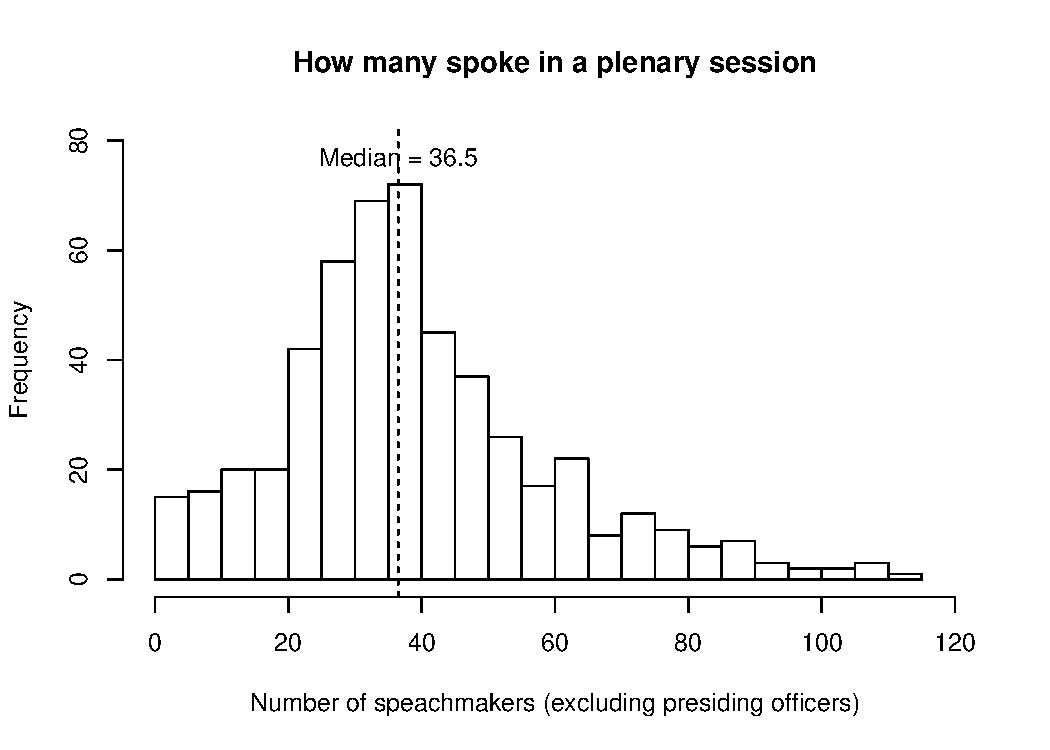
\includegraphics[width=.8\columnwidth]{../plots/nspeakers.pdf}
\end{figure}


\subsection{By legislatura}

\singlespacing
\begin{footnotesize}
\begin{verbatim}
* * Descriptives by legislatura * *
> print(round(summ,0))
  Group.1 nword.day.50% nword.day.90% nword.day.max nspeakers.day.50%
1      60           652          1215         15932                26
2      62           611          1254          9765                38
3      64           547           975          6358                56
  nspeakers.day.90%
1                45
2                61
3                81
\end{verbatim}
\end{footnotesize}
\doublespacing

\section{Stuff from urge.tex follows}

\section*{A Model of Urgency-as-Fast-Track Authority}

\begin{figure}
  \centering
    \caption{The president rules game}\label{F:game}
    \tikzstyle{mid}=[circle,draw]
    \begin{tikzpicture}
      \node[mid] at (1.5,-0.25) (c) {\emph{C}};
      \node[mid] at (4,1) (p) {\emph{P}};
      \node[mid] at (6.5,-0.25) (f) {\emph{F}};
      \node at (4,-1.5) (ce) {$q$};
      \node at (6.5,2.25) (pe1) {$x_F$};
      \node at (9,1) (fe1) {$x_C$};
      \node at (9,-1.5) (fe2) {$q$};
      \path[-] (c) edge node [above, sloped] {\footnotesize{report}} (p)
               (p) edge node [above, sloped] {\footnotesize{fast}} (f)
                   edge node [below, sloped] {\footnotesize{track}} (f);
      \path[] (c) edge node [below, sloped] {\footnotesize{$x_C$}} (p);
      \path[-o] (c) edge node [below, sloped] {\footnotesize{not}} (ce)
                (p) edge node [above, sloped] {\footnotesize{standard}} (pe1)
                (f) edge node [above, sloped] {\footnotesize{accept}} (fe1)
                    edge node [below, sloped] {\footnotesize{reject}} (fe2);
      \path[-o] (p) edge node [below, sloped] {\footnotesize{considerat.}} (pe1);
    \end{tikzpicture}
\end{figure}

\begin{description}
  \item [Hypothesis 1:] Presidents are more likely to fast-track bills when the committee chair with jurisdiction over the bill  belongs to the president's party than otherwise.
\end{description}

\section*{Data and Analysis}

We collected original data to test the hypothesis, compiling bill histories of every draft law that the executive introduced in Congress between 1998 and 2014:\footnote{We scraped the \emph{C\'amara de Diputados'} web page (\url{www.camara.cl}) in November 2014 to retrieve the record (\emph{bolet\'in}) of every proposal made between 11 March 1998 and 10 March 2014, inclusive. Data and commented code for replication accompany the online appendix. We conducted data analysis with a multiplicity of \texttt{R}'s libraries.} when each was introduced, in which chamber of the bicameral Congress, the issue it deals with, the status at the time of consultation, and so forth. We also gathered information on the chronological detail of the bill's legislative process in the House: committee referrals and reports, floor discussion and voting, when it was sent to the Senate, and more. Of direct relevance, we coded all bills marked urgent in the \emph{C\'amara de Diputados}. Earlier years antedate Internet publication and were dropped, as data completeness in the primary source remains to be verified. The period selected fully covers two Senates, four \emph{C\'amaras}, and three presidencies (plus the last two years of an earlier presidency).

\begin{table}
\centering
\caption{Proposals, legislation, and fast-track authority}\label{T:billDescriptives}
\begin{tabular}{llrr}
\multicolumn{4}{c}{\textbf{Part A. Executive bills}} \\
   & \multicolumn{2}{l}{Bills}                           &   frequency  \\ \hline
I  & \multicolumn{2}{l}{introduced}                      &       1,467  \\ \hdashline
II & \multicolumn{2}{l}{passed}                          &       1,059  \\
   & \multicolumn{2}{l}{as \% of introduced}             &   \emph{72}  \\ \hdashline
III& \multicolumn{2}{l}{fast-tracked}                    &         540  \\
   & \multicolumn{2}{l}{as \% of introduced}             &   \emph{37}  \\ \hdashline
IV & \multicolumn{2}{l}{fast-tracked \& passed}          &         415  \\
   & \multicolumn{2}{l}{as \% of fast-tracked}           &   \emph{77}  \\ \hline
\\
\multicolumn{4}{c}{\textbf{Part B. Urgent bills by presidency}} \\
\multicolumn{2}{l}{President and period}    & $N$ bills & \% fast-tracked \\ \hline
\multicolumn{2}{l}{Frei 1998--2000$^\dagger$} & 128       &  \emph{38} \\
\multicolumn{2}{l}{Lagos 2000--2006}        & 544       &  \emph{25} \\
\multicolumn{2}{l}{Bachelet 2006--2010}     & 392       &  \emph{39} \\
\multicolumn{2}{l}{Pi\~nera 2010--2014}       & 403       &  \emph{50} \\ \hdashline
\multicolumn{2}{l}{All 1998--2014}          & 1,467     &  \emph{37} \\
\hline
\multicolumn{4}{r}{\footnotesize{$^\dagger$ Last third of the six-year term in the analysis only.}} \\
\end{tabular}
\end{table}

Table \ref{T:billDescriptives} offers a general summary of bill introductions, passages, and fast-track incidences. The executive sent 1,467 bills to Congress between 1998 and 2014, on average ninety-one yearly. (Members of Congress proposed 79 percent of all bills, not analyzed.) More than one thousand proposals became law during the period, putting the executive's success rate at 72 percent---high by Latin American standards \citep{morgenstern.nacif.2002}. And 540 bills were on the fast-track during lower chamber consideration, 37 percent of all bills introduced. And 77 percent of those became law, so about 40 percent of bills that became law did it under restrictive procedures. 

The variance in urgency incidence across administrations, reported in part B, is considerable. But differences in urgency authority usage do not seem related with specifics traits of the president. For instance, one could argue that presidents with previous legislative experience might be less inclined to interfere with Congressional priorities. Frei (with previous legislative experience) and Bachelet (without) were about on average, Lagos (with experience) quite below, and Pi\~nera (without) quite above.

\subsection*{Fast-Track predictors}

Multivariate analysis of the data is revealing. The unit of analysis is individual executive proposals: the dependent variable \emph{Fast-tracked Bill} equals 1 for proposals marked with `supreme urgency' while in the C\'amara, 0 otherwise. Our main independent variable accounts for preference coincidence between the president and the reporting committee. We include controls for bill features, for timing, and for the strategic environment. Formal variable definitions and descriptive statistics appear in the online appendix.

With respect to our main independent variable, which accounts for preferences, we include \emph{Co-partisan Chair} and \emph{Coalition Chair}, which seek to identify committee chairs' preference location vis-\`a-vis the president, and \emph{Multiple Referrals}, which identifies bills referred to multiple committees. \emph{Co-partisan Chair} equals 1 if the bill was referred to a standing committee presided by a member of the president's party, and equals 0 otherwise; \emph{Coalition Chair} equals 1 for bills referred to committees chaired by members of any party in the presidential coalition, 0 otherwise. These are two different ways in which we measure our key explanatory variable, spatial proximity between the chief executive and the reporting committee, and we expect each to associate positively with the dependent variable. Part A of Table \ref{T:chairsSeats} shows that the number of standing committee chairs in hands of the president's party varied in the period, from a high of 53 percent in the 1998--2002 legislature to a low of 17 percent in 2006--10. And the opposition chaired no standing committee in 2006--10, but up to 24 and 27 percent in 2002--06 and 2010--14, respectively.\footnote{\emph{Largesse} towards opposition parties was probably aimed at beefing up the president's legislative support. Unlike the Senate, the coalition remained in control of the C\'amara throughout the period. But, by requiring 67, 60, and 57 percent votes of each chamber, respectively, constitutional reform, constitution-interpreting legislation, and organic laws therefore always required support across the aisle.}

\begin{table}
\centering
\caption{The president's status in Congress and its committees. Percent chairs/seats by party. The president's coalition in 1998--2010 was Concertaci\'on; it was Alianza afterwards. Regional includes major-party splinters (from Christian Democrats and UDI). President's status in the Senate slightly and briefly oscillated above and below majority due to vacant seats. Source: prepared with information from \protect\url{www.camara.cl}.}\label{T:chairsSeats}
\begin{tabular}{lrrrr}
                      & 1998--2002 & 2002--06 & 2006--10 & 2010--14 \\ \hline
\mc{5}{c}{\textbf{~~Part A. Committee chairs, C\'amara}} \\
President's party     &  \emph{53} & \emph{35}  & \emph{17}  & \emph{23}   \\
Other coalition party &  \emph{41} & \emph{41}  & \emph{83}  & \emph{50}   \\
Opposition            &   \emph{6} & \emph{24}  &            & \emph{27}   \\ \hdashline
Total                 & \emph{100} & \emph{100} & \emph{100} & \emph{100}  \\ 
$N$ standing committees&  17        &  17      &  18      & 22      \\ [1.8ex] \hline 
\mc{5}{c}{\textbf{~~Part B. Seats, C\'amara}} \\ 
President's coalition & \emph{58}     & \emph{53}  & \emph{51}   & \emph{50}   \\
Opposition            & \emph{42}     & \emph{48}  & \emph{47}   & \emph{48}   \\
Regional              &               &            & \emph{3}    & \emph{2}    \\ \hdashline
Total       & \emph{100}    & \emph{100} & \emph{100}  & \emph{100}  \\ [1.8ex] \hline
\mc{5}{c}{\textbf{~~Part C. Seats, Senate}} \\
President's coalition & \emph{50}            & \emph{50}       & \emph{55}   & \emph{45}       \\
Opposition            & \emph{50}            & \emph{50}       & \emph{45}   & \emph{55}       \\ \hdashline
Total                 & \emph{100}$^{\dagger}$ & \emph{100}      & \emph{100}  & \emph{100}      \\ \hline
\mc{5}{r}{\footnotesize{$^\dagger$vacant seats dropped}}
\end{tabular}
\end{table}

We also control for multiple referrals. Nearly one quarter (24 percent) of bills in the period were referred to more than one standing committee. The ``other committee'' count excludes the Finance Committee, with jurisdiction over any form of new spending (and discussed next---multiple referrals reach 32 percent when the Finance Committee is considered). Also excluded are special and bicameral committees. \emph{Multiple Referrals} should capture any effect of agenda control sharing among several committee chairs during the proposal's negotiation---reflecting the need to rein on unruly chairs through a friendlier committee. A single co-partisan or coalition chair among multiple referees suffices for the indicator previously discussed to equal 1. 

The variable intended to capture bill-specific features is \emph{Hacienda Referral}, which equals 1 for bills referred to the powerful Finance Committee with special status in the Chilean Congress, 0 otherwise. Unlike other standing committees, the Finance Committee has jurisdiction over \emph{every} bill authorizing spending in any domain. Moreover, the unanimous exception rule discussed earlier is inapplicable to \emph{Hacienda} bills, which must be reported prior to floor consideration.\footnote{\emph{Ley Org\'anica del Congreso} arts.\ 17 and 21.} Committee members, working in tandem with the Finance Ministry, may or may not appropriate funds from the budget in their report \citep{aleman.navia.UrgChi.2009}. Not unlike the Appropriations and Rules committees in the U.S.\ House, \emph{Hacienda} has the status of a control committee, a key asset for agenda power \citep{kiewiet.mccubbins.1991}. \emph{Hacienda} referral therefore controls for a subset of generally important proposals, and we expect it to associate positively with urgency authority.

Three controls account for the strategic environment. \emph{Presidential Approval} is the net general population presidential approval rate at bill initiation (i.e., the percentage of respondents who approve of the president's job minus the percentage who disapprove). We have no a priori expectation here. If presidents with better public opinion standing are also more successful in the legislative arena \citep{bond.fleisher.1990,aleman.navia.UrgChi.2009}, they might also need restrictive rules less often, and reliance on the fast-track might therefore drop (in some issue areas, at least).\footnote{We estimate the models using subsets of bills by issue area in the online appendix. Smaller numbers of bills tend to hamper statistical significance, but the results are in line with those reported.} The contrary might hold if popular presidents were more successful in obtaining more likeable reports from the average committee chair, that would then require protection against floor amendments. \emph{Introduced in Senate} equals 1 for bills sent to the Upper Chamber, 0 otherwise. By virtue of being smaller, enjoying longer terms, and not being firmly under the president's coalition control during most of the period, bills sent to the Senate might present systematic differences in fast-track usage. And \emph{Senate Majority} equals 1 if the president's coalition controlled half or more of Upper Chamber seats when the bill was initiated, 0 otherwise.\footnote{Parties in the presidential and opposition coalitions were tied throughout most of the 1998--2006 Senate (majority briefly oscillating back and forth in the first years due to member indictments, impeachments, and deaths in both coalitions). Ties are coded as \emph{Senate Majority} = 1.} Other things equal, presidents with sufficient partisan legislative resources in both chambers will find it easier to push proposals through Congress, and might be less inclined to use the fast-track prerogative to successfully navigate log-rolls through the plenary session.

The group of variables accounting for time-related effects control for different aspects of the congressional cycle. \emph{Year Remaining} (and its squared value to capture non-linearity, if any) measures the percentage of the legislative year remaining at bill initiation. Chilean legislative years start after the (meridional) summer break. So the variable adopts value 100 for proposals introduced on March 1 (the first day of the legislative year), and value 0 for proposals introduced the last day of February. It should control for stationarity in the data (the online appendix elaborates the temporal dimension in the use of urgencies). And \emph{Relax Deadline} equals 1 for bills initiated in July 2010 or later, 0 otherwise. Congress doubled deadlines to consider and vote urgent bills five months into the 2010--14 legislature (see online appendix). Any systematic shift in urgency usage attributable to this reform should be reflected in this coefficient. 

\subsection*{Model Specification and Results}

Given that we pool observations from four elected legislatures, with important differences in the types and the volume of proposals considered \citep{aleman.navia.UrgChi.2009}, heterogeneity might interfere. We fit two additional model specifications for robustness verification. One includes fixed legislature effects---i.e., three dummies for bills initiated in the 2002--06, 2006--10, and 2010--14 periods, respectively; the excluded 1998--2002 dummy is the baseline. Another adds further flexibility by also estimating separate errors for bills initiated in each legislature \citep[a so-called mixed effects model,][, 262, 302]{gelman.hill.2007}. We rely on a generalized linear model for mixed effects estimation, and logit for the rest. We normalized continuous variables \emph{Presidential Approval} and \emph{Year Remaining} to speed the GLM's convergence.\footnote{As suggested in \url{http://stackoverflow.com/questions/23478792/warning-messages-when-trying-to-run-glmer-in-r} and \url{https://rstudio-pubs-static.s3.amazonaws.com/33653_57fc7b8e5d484c909b615d8633c01d51.html}. Normalization re-scales and centers the measures in order to improve parameter identification.} Normalized measures were used throughout for model comparability.

% Table created by stargazer v.5.2 by Marek Hlavac, Harvard University. E-mail: hlavac at fas.harvard.edu
% Requires LaTeX packages: dcolumn 
\begin{table}
  \centering 
  \caption{Executive bill fast-track predictors. Standard errors in parentheses. Model 3 includes fixed Legislatura effects (not reported). Model 4 estimates separate error terms by Legislatura. Method of estimation: model 4 with generalized linear model, others with logit \citep[fitted with \texttt{R} base's \texttt{glm} and library \texttt{lme4},][]{lme4.2015}.}\label{t:urgenLogit}
  \begin{tabular}{@{\extracolsep{0pt}}lD{.}{.}{-3} D{.}{.}{-3} D{.}{.}{-3} D{.}{.}{-3} } 
    \hline \\[-1.8ex] 
    & \multicolumn{4}{c}{DV: Bill on fast-track (1) or not (0)} \\ 
    \\[-1.8ex] & \multicolumn{1}{c}{(1)} & \multicolumn{1}{c}{(2)} & \multicolumn{1}{c}{(3)} & \multicolumn{1}{c}{(4)}\\ 
    \\ [-1.8ex] 
    \hline \\[-1.8ex] 
    \emph{Co-partisan}     &  .289^{**}   &  &  &                                   \\
    \emph{Chair}           & (.024)      &  &  &                                   \\ [.75ex]
    \emph{Coalition}       &             & .825^{***}   & .874^{***}    & .847^{***}   \\
    \emph{Chair}           &             & (.005)      & (<.001)     & (<.001)     \\ [.75ex]
    \emph{Multiple}        &  .772^{***}  &  .795^{***}  &  .808^{***}   &  .809^{***}   \\
    \emph{Referrals}       & (<.001)     & (<.001)     & (<.001)     & (.004)      \\ [.75ex]
    \emph{Hacienda}        & 1.002^{***}  & .940^{***}   & .917^{***}    & .923^{***}    \\
    \emph{Referral}        & (<.001)     & (<.001)     & (<.001)     & (<.001)     \\ [.75ex]
    \emph{Pres.}           &  -.078      &  -.096      &  .029       & -.044       \\
    \emph{Approval}        & (.286)      & (.187)      & (.710)      & (.567)      \\ [.75ex]
    \emph{Introduced}      &  -.716^{***} &  -.698^{***}  &  -.744^{***} &  -.730^{***}  \\
    \emph{in Senate}       & (<.001)     & (<.001)     & (<.001)      & (<.001)    \\ [.75ex]
    \emph{Senate}          &  -.251      &  -.319      &             &             \\
    \emph{Majority}        & (.214)      & (.110)      &             &             \\ [.75ex]
    \emph{Year}            &  .072       &  .065       &  .053        &  .053      \\
    \emph{Remaining}       & (.223)      & (.268)      & (.370)       & (.368)     \\ [.75ex]
    \emph{(Year}           &  -.224^{***} &  -.238^{***}  &  -.255^{***}  &  -.251^{***} \\
    \emph{Remaining)$^2$}  & (<.001)     & (<.001)      & (<.001)     & (<.001)    \\ [.75ex]
    \emph{Relax}           &  .479^{*}    &  .394       &              &            \\
    \emph{Deadline}        & (.057)      & (.104)      &              &            \\ [.75ex]
    %% \emph{2002-06 Leg.} &  &  &  -.203 &                                        \\
    %%                     &  &  & (.298) &                                        \\ [.75ex]
    %% \emph{2006-10 Leg.} &  &  &  .302^{*} &                                     \\
    %%                     &  &  & (.097) &                                        \\ [.75ex]
    %% \emph{2010-14 Leg.} &  &  & 1.200^{***} &                                   \\
    %%                     &  &  & (<.001) &                                       \\ [.75ex]
    Intercept              &  -1.046^{***} & -1.589^{***} & -1.933^{***} & -1.719^{***}  \\
                           & (<.001)      & (<.001)     & (<.001)    & (<.001)     \\ [.75ex]
    \hline \\[-1.8ex] 
    Effects & \multicolumn{1}{c}{none} & \multicolumn{1}{c}{none} & \multicolumn{1}{c}{fixed} & \multicolumn{1}{c}{mixed} \\ 
    Observations & \multicolumn{1}{c}{1,467} & \multicolumn{1}{c}{1,467} & \multicolumn{1}{c}{1,467} & \multicolumn{1}{c}{1,467} \\ 
    Log$L$ & \multicolumn{1}{c}{$-864$} & \multicolumn{1}{c}{$-862$} & \multicolumn{1}{c}{$-852$} & \multicolumn{1}{c}{$-859$} \\ 
    \% correct & \multicolumn{1}{c}{67} & \multicolumn{1}{c}{68} & \multicolumn{1}{c}{68} & \multicolumn{1}{c}{68} \\ 
%%Akaike Inf. Crit. & \multicolumn{1}{c}{1,748.896} & \multicolumn{1}{c}{1,740.400} & \multicolumn{1}{c}{1,719.057} & \multicolumn{1}{c}{1,731.050} \\ 
%%Bayesian Inf. Crit. &  &  &  & \multicolumn{1}{c}{1,778.632} \\ 
    \\ [-1.8ex] 
    \hline \\[-1.8ex] 
    & \multicolumn{4}{r}{\footnotesize $^{*}$p$<$.1; $^{**}$p$<$.05; $^{***}$p$<$.01 (p-values in parentheses)} \\ 
  \end{tabular} 
\end{table} 

Table \ref{t:urgenLogit} reports results.\footnote{The regression model performs satisfactorily. A likelihood-ratio test of overall fit rejects the hypothesis, at below the .001 level, that an intercept-only fit is as good as our models. Predictors across model specifications correctly classify 67--68 percent of the observations.} We find support for our main hypothesis. In line with expectations, both variables measuring the proximity of committee chairs to the president increase the probability of fast-track. \emph{Co-partisan Chair} has a positive coefficient in model 1, as hypothesized, and the effect achieves conventional statistical significance (parentheses in the table report p-values). The evidence is much stronger for the variable's other specification: the coefficient for \emph{Coalition Chair} in models 2--4 is also positive, triples its size, and achieves p-values at .005 or below. In other words, if a bill is referred to a committee where the president finds support (either because the chair belongs to her party or to her coalition), the report is more likely to be fast-tracked for floor consideration. This matches previous scholarship, i.e., that the coalition is as good a predictor of presidential support in Congress---or better, in our case---as the party. The finding is robust across model specifications. In general, all model coefficients remain pretty much unchanged in size and significance when fixed and mixed effects are included on the right side (\emph{Senate Majority} and \emph{Relax Deadline} must be dropped due to colinearity with legislature dummies). 

%% > mar3
%%      factor     AME     SE       z      p   lower   upper
%%   dsameCoal  0.1734 0.0585  2.9651 0.0030  0.0588  0.2880
%%   dmultiRef  0.1603 0.0250  6.4003 0.0000  0.1112  0.2093
%%     drefHda  0.1817 0.0232  7.8483 0.0000  0.1363  0.2271
%%  netApprovR -0.0030 0.0153 -0.1976 0.8433 -0.0331  0.0270
%%      dinSen -0.1475 0.0335 -4.3981 0.0000 -0.2132 -0.0818
%%      legyrR  0.0173 0.0120  1.4463 0.1481 -0.0062  0.0408
%%     legyrR2 -0.0535 0.0127 -4.2213 0.0000 -0.0784 -0.0287
%%   legis2002 -0.0628 0.0374 -1.6802 0.0929 -0.1360  0.0105
%%   legis2006  0.0525 0.0370  1.4185 0.1561 -0.0200  0.1249
%%   legis2010  0.1813 0.0389  4.6590 0.0000  0.1050  0.2575

%% \begin{figure}
%%   \centering
%%     \caption{Average marginal effects from model 3. Dots report how the probability of an urgent bill changes in response to a unit change in each independent variable, all else at mean values; bars are 95-percent confidence intervals.}\label{F:avgMg}
%%     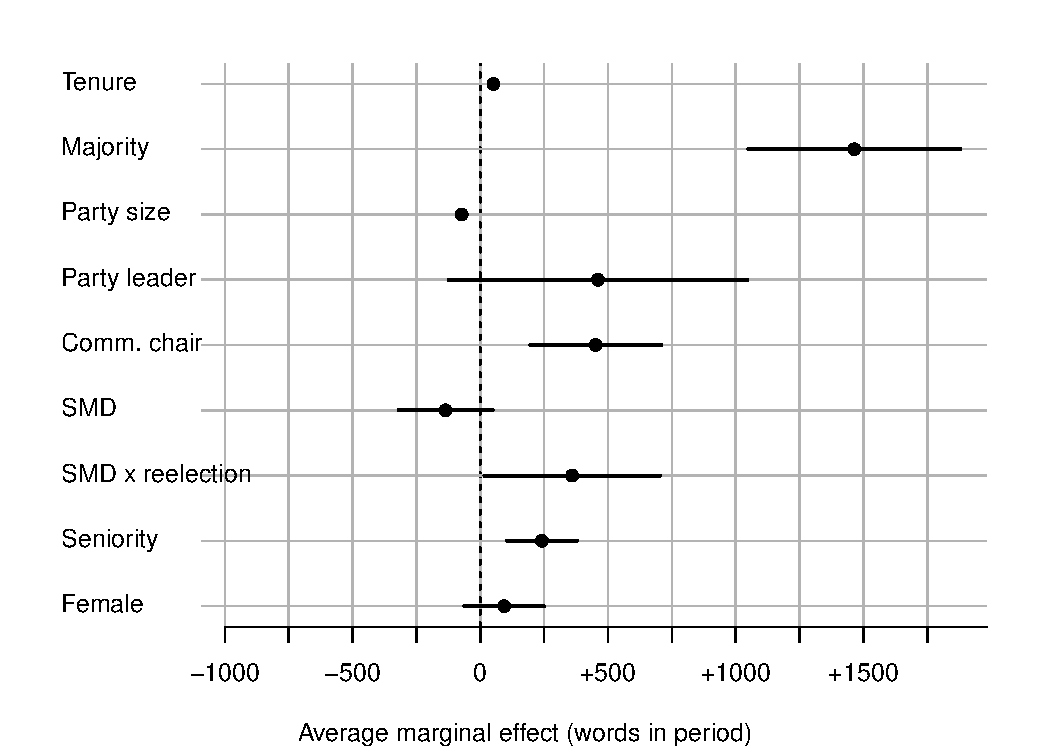
\includegraphics[width=.8\columnwidth]{../graphs/avgMgEffects.pdf}
%% \end{figure}

Figure \ref{F:avgMg} reports changes in the average predicted probability that a bill is fast-tracked associated with unit changes in model 3's explanatory variables (all other regressors at their mean value). This is a convenient way to gauge logit regression coefficients, by translating them into interpretable quantities. The report from a committee with a coalition chair experiences a 0.17 hike (0.06 standard error) in the likelihood of receiving a closed rule compared to a report by an opposition-chaired committee. The effect is as big as the average marginal effects of \emph{Hacienda Referral} (0.18), which capures mostly high-significance draft laws, and that of \emph{Multiple Referrals} (0.16), which we view as an indicator of issue complexity. We therefore find no statistical evidence to reject our Hypothesis 1. The results also confirm hypothesis 2, showing that a bill reported by a generally less friendly committe (chaired by the opposition), has a higher probability of receiving an open rule on the floor, thereby allowing the floor majority to bring back the bill to the median through floor amendments. Thus, presidents use open rules to control bills coming from preference distant committee chairs.

The substantial effects of \emph{Hacienda Referral} and \emph{Multiple Referrals} deserve comment. They suggest, first, that when spending gets in the way, restrictive rules are the norm in Chile. Recall that \emph{Multiple Referrals} exclude the Finance Committee, so there is an independent effect of bills with jurisdictional overlaps worth investigating further, and which must be associated, in part at least, to influencing the report through a friendlier committee.\footnote{We are grateful for this insight from an anonymous referee. According to \citet[][, 118]{sotoCongChile2015}, multiple-referees may act sequentially or in tandem, as decided by the C\'amara's presiding officer. When sequential, a divergent secondary committee's report is treated as an amendment to the primary committee's---an urgency overrides the secondary (and subsequent) report(s). We unfortunately lack information on this important aspect of multiple referrals.} Furthermore, note that the Finance Committee was always chaired by a coalition member but, with the exception of the 1998--2000 period, never by a co-partisan of the president. This may explain the milder effect of the partisan specification of our key variable in model 1. 

Another effect worth highlighting is \emph{Introd.\ in Senate}. Bills successfully passing the Upper Chamber first, where the opposition was systematically larger and at times in control, were much less likely to get urgent status (the average marginal effect is $-0.15$ and significant). This suggests that agreements and compromises reached in the Senate ignited less, not more, protection from floor amendments in the \emph{C\'amara's} plenary, most likely as a consequence of the greater preference divergence between the President and the opposition-led Senate. Analysis of inter-chamber negotiation and the reliance on urgency in the Upper Chamber are interesting venues for future research. 

%% \begin{figure}
%%   \centering
%%     \caption{Probability of fast-track bill consideration. Predictions are from from model 3 letting \emph{Year Remaining} vary in full range, with 95\% confidence bands. Other variables set at the following values: $\text{\emph{Multiple Referrals}}=0$, $\text{\emph{Hacienda Referral}}=0$, $\text{\emph{Introd.~in~Senate}}=0$, $\text{\emph{2006-10}}=1$, and $\text{\emph{Pres.~Approval}}=.33$ (Bachelet's mean).}\label{F:sims}
%%     \includegraphics[width=.75\columnwidth]{../graphs/predictedPr.pdf}
%% \end{figure}

Finally, there are time trends in fast-track authority that simulations reveal neatly. Figure \ref{F:sims} portrays the predicted probability that a bill enters the fast-track throughout the legislative year. Regressors in model 3 are held constant to simulate a bill sent to the \emph{C\'amara} in the 2006--10 Legislature that was referred to a single committee, excluding \emph{Hacienda}. \emph{Presidential Approval} (insignificant across models) is set to the mean for President Bachelet's first term, coinciding in full with the 2006--10 Legislature. The inverted-U shape shows how fast-track probability, predicted at 0.17 for coalition-chaired committees at the start, and 0.08 for the rest, becomes much likelier in the first half of the legislative year. By the second quarter (June--August), the probability is at its peak, about 0.32 percent and 0.17, respectively. It then experiences a sharp drop, ending the austral Summer break at 0.13 for coalition-chaired committees, and 0.05 for others. And while 95-percent confidence bands overlap, they barely do so at the middle of the legislative year, lending confidence that we are picking up a signal and not just random noise. 

\section*{Discussion}\label{s:discussion}

This paper has argued that beyond the effect of urgency authority on the timing and deadlines for bill consideration, its procedural effects conceal a much more significant effect, by allowing presidents to shield desired policy from amendments on the floor. Furthermore, the president's decision not to use this tool is also important. An open rule means that bills can receive amendments on the floor that may move it closer to the president's preferences. This paper portrays urgency authority, found in seven Latin American constitutions, as equivalent to the fast-track authority that United States presidents enjoy periodically. Doing so shows how proposals that presidents qualify as urgent are considered under restrictive rules by the chamber's plenary: they must be voted up-or-down, without amendments.

While all seven constitutions remain silent about the procedural implications of urgency authority, and we have only looked for these restrictive procedures in statutes and chamber rules in the case of Chile, there are good reasons to expect that other countries have included similar provisions. After all, the rationale of the urgency authority is expediting the legislative process, and restrictive rules are a natural choice to speed urgent bills' consideration before an explicit deadline expires. 

The classification of constitutional urgency authority into the plenary arrest (Brazil), automatic adoption (Ecuador, Paraguay, Uruguay), and indeterminate (Chile, Colombia, Mexico) variants, which we presented in Section 2, naturally brings two pending issues to the fore. One is cross-national validation of the presence of restrictive procedures at the level of statutes or chamber rules---especially where urgency effects are seemingly indeterminate, as in Chile. The task ahead is to identify procedures that restrict the choices available to legislators, such as closed rules do in Chile. The other is the need to model the bargaining logic of plenary-arrest and automatic-adoption variants in search of similarities and differences with the urgency-as-fast-track. We expect these efforts to generalize our argument beyond Chile, our case study.

Game-theoretic treatment of urgency-as-fast-track authority shows that preference overlap between the president and the reporting committee is the mechanism driving the choice to put bills on the fast-track. The reverse also applies: bills referred to opposition-chaired committees, who might report them to the floor with fundamental changes, are less likely to be fast tracked. The president would prefer them to go to the floor with an open rule, especially if on the floor a (friendlier) majority can restore the original intent of the president and her party. Systematic analysis of proposals in the Chilean lower chamber in recent years yields evidence that, other things constant, bills reported by committees chaired by members of the president's coalition/party are about twice as likely to be fast-tracked than the rest. To the extent that parties and coalitions indicate preference overlap (as is accepted in Chile), the evidence supports our main theoretical result.

The paper's results and findings are of natural interest to students of comparative political institutions, especially those interested in legislative procedure and separation of powers. They also shed light on the field of American Politics. In a provocative book, \citet{howell.moe.Relic2016} make an argument in favor of giving U.S.\ presidents permanent fast-track authority not limited to trade agreements. In order to have a coherent and effective government, they argue in favor of constitutional reform to put the executive at the center of the legislative process: ``presidents should be granted enhanced agenda-setting powers to propose bills to Congress, which Congress should then be required to vote on without amendment, on a strictly majoritarian basis, within a fixed period of time'' \citep[][, 145]{howell.moe.Relic2016}. Failure to vote in due time would turn those bills into law. Equating urgency and fast-track authorities shows this to be the automatic adoption variant. Reform would therefore make U.S.\ presidents similar to those in Ecuador, Paraguay, and Uruguay in this respect. 

Our results also speak to students of executive decrees and unilateral policymaking more generally. As discussed at the start of the paper, urgency authority and decree authority may overlap, as in fact they do in Brazil, Chile, and Colombia. We have established that, while urgency authority increases the president's leverage over the legislative process, an agreement is needed between the president and her congressional allies without which this prerogative is rendered powerless. Congress retains authority to reject urgent proposals, and cannot therefore be made worse-off than the status quo. Executive decrees, on the other hand, imply an abdication of decision rights on the part of legislators to participate in the process, and force legislators to respond to the president's enacted decree instead once it has already altered the status quo.

Yet for this precise reason executive decrees are not a true alternative in certain cases \citep{palanza.2019}. \citet[][, 164]{figueiredo.limongi.2000} report that urgent bills in Brazil are quite rare since the provisional decree ``is a much more efficient way of speeding up and approving legislation.'' More research should be done to establish whether effectively the urgency prerogative is used, for instance, on issues that are excluded from executive decree authority in the Brazilian constitution. Previous findings indicate that reliance on decrees effectively diminishes when policy deals with these issues---although it does not disappear. It is undeniable that Chile, where executive decrees are seldom used (only two decrees have been enacted since 1990), resorts to urgency authority expansively. Future research, and hopefully comparative work, will help tackle this issue. 

Chilean legislative scholars will find interest in investigating a missing piece in our argument. To be clear, the research advanced in this paper sheds light on the factors that affect the likelihood of reliance on urgency authority, and we provide an argument explaining the mechanism that leads to this usage. But we do not provide verification that closed rules do in fact dispel amendments---a key and untested premise of our approach. Systematic contrasting of bills that presidents drafted in the period, the various amendments that were introduced, the committee reports, and the text ultimately adopted, would enable analysts to demonstrate whether or not urgencies in fact dodge amendments. This is a difficult but promising venue for future research. 

Last, we emphasize that our investigation contributes to the literature on restrictive procedures. To the general class of procedures as instruments of political control, we add the urgency authority. One difference sets fast-track mechanisms apart from standard closed rules. Standard restrictive rules give agenda power to legislators---it may be the plenary \citep{mcnollgast.1987}, standing committees \citep{weingast.1992}, the bicameral conference \citep{shepsle.weingast.1987}, or the majority party \citep{cox.mccubbins.1997}. Urgency puts the executive in control of protecting vulnerable legislative agreements. The unique role and function to determine whether or not a major bill will be considered in the U.S. House, and which amendments and motions will be allowed, is firmly in control of the legislative leadership, acting as sole gatekeepers to the plenary \citep{cox.2006}. As with France's \emph{vote bloqu\'e} \citep{huber.1996b}, fast-track authority lets the executive branch pull some of the gatekeeping levers, earning a priceless legislative prerogative worthy of further research.

\section*{Acknowledgements}
The author is grateful to xxx for research assistance. Eric Magar received financial support from the Asociaci\'on Mexicana de Cultura \textsc{a.c.}\ and \textsc{conacyt}'s Sistema Nacional de Investigadores. The authors are responsible for mistakes and shortcomings in the study.

\listofendnotes

\bibliographystyle{apsr}

\bibliography{../bib/magar}

%% \begin{thebibliography}{xx}

%% \harvarditem{Alem\'an \harvardand\ Tsebelis}{2016}{aleman-tsebelis-2016-book}
%% Alem\'an, Eduardo \harvardand\ George Tsebelis. 2016.
%% \newblock {\em Legislative Institutions and Lawmaking in Latin America}.
%% \newblock Oxford:  Oxford University Press.

%% \harvarditem{Alem\'an \harvardand\ Navia}{2009}{aleman.navia.UrgChi.2009}
%% Alem\'an, Eduardo \harvardand\ Patricio Navia. 2009.
%% \newblock ``Institutions and the Legislative Success of `Strong' Presidents: An
%%   Analysis of Government Bills in {Chile}.'' {\em Journal of Legislative
%%   Studies} 15(4):401--19.

%% \end{thebibliography}


\end{document}

